% RiskShip -- solución con programación genética, formato IEEE (conferencia).
% Compilar con pdfLaTeX:
%   cd papers && Rscript -e 'tinytex::pdflatex("riskship_gp.tex")'
% En Overleaf: subir este archivo y la carpeta figuras/.
%
% Todas las cifras del GP provienen de results/gp_full_v1/ (final_metrics.csv,
% summary.json, configuration_selection.json, selection_sealed_before_test.json,
% domain_purity_audit.json, timing_anomalies.json, *_history.csv, los JSON por
% corrida) y de docs/GP_ENTRENAMIENTO_COMPLETO.md; las de la RNA, de README.md
% ("Experimental protocol and results") y del informe informe/riskship_rna.tex.
% La figura figuras/rna_gp_comparison.png es la que el notebook ejecutado
% notebooks/gp_shipment_loss.ipynb muestra desde
% results/gp_full_v1/figures/rna_gp_comparison.png; no se edita a mano.
\documentclass[conference]{IEEEtran}

\usepackage[utf8]{inputenc}
\usepackage[T1]{fontenc}
\usepackage[spanish,es-tabla,es-nodecimaldot,es-noshorthands]{babel}
\usepackage{amsmath}
\usepackage{array}
\usepackage{booktabs}
\usepackage{cite}
\usepackage{graphicx}
\usepackage{url}

\graphicspath{{figuras/}}

% Nombres de columnas del conjunto de datos (admite guiones bajos).
\newcommand{\col}[1]{\texttt{\detokenize{#1}}}

\renewcommand{\IEEEkeywordsname}{Palabras clave}

\begin{document}

\title{RiskShip: Priorización Inteligente de Envíos con Riesgo de Falla\\
{\large Solución con programación genética}}

\author{\IEEEauthorblockN{Kevin Bueno S. y Lizeth Portela L.}
\IEEEauthorblockA{\textit{Departamento de Ingeniería, Pontificia Universidad Javeriana}\\
Bogotá D.C., Colombia\\
bueno.kevin@javeriana.edu.co, portelali@javeriana.edu.co}}

\maketitle

\begin{abstract}
RiskShip es un agente de priorización que estima el riesgo de pérdida de un
envío en el momento de su creación, antes del despacho, y ordena los casos para
que un equipo con capacidad limitada revise primero los más críticos. Este
artículo presenta la segunda técnica del proyecto: un clasificador simbólico
evolucionado con programación genética (GP) sobre el mismo conjunto de datos,
las mismas 13 variables y la misma partición temporal que la red neuronal
(RNA) de referencia. Los árboles, construidos con DEAP a partir de operaciones
aritméticas protegidas sobre variables codificadas, se evalúan con la precisión
promedio sobre las 125\,082 filas de entrenamiento penalizada por tamaño; la
configuración, el árbol y el umbral se eligen solo en validación y la selección
se sella antes de puntuar la prueba. Con cinco semillas, el GP alcanza en el mes
de prueba un PR-AUC de 0,639~$\pm$~0,034 y un ROC-AUC de 0,773~$\pm$~0,019,
frente a 0,750~$\pm$~0,002 y 0,824~$\pm$~0,002 de la RNA sobre el mismo
\textit{holdout}: no la alcanza, pero produce expresiones de 9 a 36 nodos
legibles. Una ablación sin el dominio del producto reduce el PR-AUC a
0,577~$\pm$~0,016, lo que confirma la dependencia de una variable con un
artefacto de extracción sospechado.
\end{abstract}

\begin{IEEEkeywords}
programación genética, regresión simbólica, priorización de riesgo, logística,
partición temporal, interpretabilidad, DEAP
\end{IEEEkeywords}

\section{Introducción}

Las plataformas de comercio electrónico operan redes logísticas en las que un
envío atraviesa centros de \textit{fulfillment}, \textit{cross-docking},
transporte intermedio y última milla~\cite{meli10k}. La capacidad humana de
monitoreo es limitada, de modo que el valor de un modelo no está solo en
clasificar bien, sino en concentrar la atención en la fracción de casos con
mayor riesgo. En la literatura, el riesgo en cadenas de suministro se ha
abordado con redes neuronales~\cite{bortolini,ye}, con lógica
difusa~\cite{gajovic,aqlan}, con mecanismos de votación~\cite{ifac2022} y con
métodos evolutivos: Nezamoddini \textit{et al.}~\cite{nezamoddini} combinan un
algoritmo genético con redes neuronales para optimizar una cadena integrada
bajo riesgo. La Sección~\ref{sec:estado} amplía esta revisión hacia la
programación genética, los datos tabulares y la evaluación bajo desbalance.

RiskShip formula el problema como una clasificación binaria (el envío se
pierde o no) resuelta a través de un puntaje continuo de riesgo que ordena los
casos. La primera entrega del proyecto resolvió esa tarea con redes
neuronales~\cite{informe_rna}. Este artículo presenta la segunda técnica:
programación genética (GP)~\cite{koza}, que evoluciona expresiones simbólicas
cuya salida es el puntaje. A diferencia de una red, el resultado es una fórmula
que puede leerse, auditarse y, si fuera necesario, calcularse a mano; a cambio,
la búsqueda es estocástica y la capacidad de representación depende de las
primitivas elegidas. La pregunta es si esa interpretabilidad se obtiene a un
costo aceptable en calidad de priorización.

\textbf{Alcance.} Igual que en la entrega anterior, la tarea se acota a
predecir la \emph{pérdida} en el \emph{momento de creación} del envío. El GP se
evalúa con el mismo protocolo que la RNA (misma limpieza, misma partición
temporal, mismo conjunto de prueba, cinco semillas y mismas métricas) para que
la comparación sea directa. La RNA no se reentrenó: sus cifras son las
publicadas en el repositorio del proyecto.

\section{Estado del arte}
\label{sec:estado}

\subsection{Programación genética para clasificación con clases desbalanceadas}

La programación genética evoluciona programas, habitualmente árboles de
expresión, mediante selección, cruce y mutación~\cite{koza}. Espejo
\textit{et al.}~\cite{espejo} revisan su aplicación a la clasificación y
distinguen tres familias: árboles de decisión evolucionados, reglas y
funciones discriminantes, que devuelven un valor numérico comparado con un
umbral. Para clases desbalanceadas, Bhowan \textit{et al.} muestran que la
exactitud como aptitud sesga la búsqueda hacia la clase mayoritaria y proponen
funciones de aptitud basadas en el área bajo la curva ROC y en la exactitud
por clase~\cite{bhowan2012}, y después un enfoque multiobjetivo que evoluciona
ensambles diversos a partir del frente de Pareto~\cite{bhowan2013}. El
clasificador de RiskShip pertenece a la familia de funciones discriminantes:
el árbol devuelve un puntaje real, el umbral se fija aparte en validación y
la aptitud es una métrica de orden (precisión promedio) en lugar de la
exactitud, en línea con esa recomendación; la aptitud multiobjetivo de esos
autores queda como trabajo futuro.

\subsection{Control del tamaño e interpretabilidad}

El crecimiento de los árboles sin ganancia de aptitud (\textit{bloat}) es un
problema clásico del GP. Luke y Panait~\cite{luke} comparan de forma
sistemática los métodos de control y concluyen que los límites estáticos de
profundidad y las penalizaciones por tamaño (presión de parsimonia) figuran
entre las técnicas más eficaces y sencillas; Poli
\textit{et al.}~\cite{poli} recogen esa práctica como estándar. Por su parte,
Rudin~\cite{rudin} sostiene que, en decisiones de alto impacto, debe
preferirse un modelo interpretable a la explicación a posteriori de una caja
negra, y La Cava \textit{et al.}~\cite{lacava} muestran en el banco de pruebas
SRBench que los métodos de regresión simbólica basados en GP alcanzan una
exactitud competitiva con modelos de caja negra con expresiones mucho más
compactas. El GP de RiskShip combina ambas ideas: límites estáticos de altura
8 y 127 nodos junto con la penalización lineal $\lambda|T|$ de la aptitud, y
el desempate por menor tamaño en la selección por validación; el resultado son
árboles de 7 a 36 nodos que se reducen a sumas ponderadas legibles.

\subsection{Redes neuronales frente a modelos de árbol y simbólicos en datos tabulares}

En datos tabulares de tamaño medio, los modelos basados en árboles siguen
superando a las redes neuronales profundas: Grinsztajn
\textit{et al.}~\cite{grinsztajn} lo atribuyen a la robustez frente a
variables no informativas y a la capacidad de representar funciones
irregulares, y Shwartz-Ziv y Armon~\cite{shwartz} comprueban que las
arquitecturas profundas propuestas para datos tabulares rara vez superan a
XGBoost fuera de los conjuntos en que fueron presentadas. Estos resultados no
se trasladan directamente al GP, cuyas primitivas aritméticas continuas se
parecen más a una red pequeña que a un árbol de decisión; la brecha de 0,110
en PR-AUC frente a la RNA sugiere que la limitación del GP de RiskShip no
proviene del tipo de datos, sino del presupuesto de búsqueda y de la ausencia
de primitivas condicionales, que es la hipótesis que motiva el trabajo futuro.

\subsection{Aprendizaje automático en riesgo logístico y pérdida de envíos}

Además de los trabajos sobre riesgo en cadenas de suministro citados en la
introducción~\cite{bortolini,ifac2022,nezamoddini}, la predicción de fallas
en la última milla se ha abordado con aprendizaje supervisado. De Leeuw
\textit{et al.}~\cite{deleeuw} predicen la pérdida de paquetes sobre un año
de envíos en Bélgica, donde la rareza de las pérdidas obliga a combinar
balanceo de clases y ensambles, y recurren a técnicas de explicabilidad a
posteriori; Zhang \textit{et al.}~\cite{zhang2026} proponen una red tabular
para el retraso en comercio electrónico y traducen las probabilidades en una
simulación costo-beneficio de la intervención. El GP en logística se ha usado
sobre todo para evolucionar políticas, como las reglas simbólicas de precios
para ventanas de entrega de Lunet \textit{et al.}~\cite{lunet}, cuyo
argumento (una política transparente y de cómputo trivial) coincide con el
del módulo GP de RiskShip. No se encontró, en cambio, un trabajo que aplique
GP a la clasificación de pérdida de envíos; la aportación de este artículo es
evaluar esa combinación bajo un protocolo temporal compartido con la RNA.

\subsection{Evaluación bajo desbalance y fuga de información}

Davis y Goadrich~\cite{davis} demuestran que una curva domina en el espacio
ROC si y solo si domina en el espacio precisión-exhaustividad, y que este
último es más informativo cuando la clase positiva es minoritaria; Saito y
Rehmsmeier~\cite{saito} confirman empíricamente que el ROC-AUC oculta
diferencias relevantes en esos casos. Kaufman \textit{et al.}~\cite{kaufman}
formalizan la fuga de información como el uso de datos que no están
legítimamente disponibles en el momento de la predicción y muestran que su
detección exige razonar sobre la cronología de cada atributo, no solo sobre
su correlación con la etiqueta. Ambas líneas sustentan decisiones del
protocolo de RiskShip: la precisión promedio como aptitud y métrica principal,
la partición temporal por mes con los terminales de codificación objetivo
calculados solo con meses anteriores, y la exclusión de las columnas de la
Tabla~\ref{tab:fuga}, entre ellas \col{DATEPARAMETER}, cuyo desfase según la
clase es precisamente una fuga de las que esos autores describen.

\section{Motivación y contextualización del problema}

\subsection{Problema de aplicación}

Mercado Envíos gestiona un volumen de paquetes en el que la pérdida real ronda
el 0,1\,\% de los envíos. Aunque la proporción es pequeña, cada pérdida
implica reembolso, reposición y deterioro de la confianza del comprador. El
equipo que puede intervenir (verificar el empaque, reforzar el seguimiento,
cambiar la ruta) tiene una capacidad fija, muy inferior al volumen diario. La
pregunta operativa no es ``¿se perderá este envío?'' sino ``¿cuáles de los
envíos creados hoy merecen la atención disponible?''. Un puntaje de riesgo que
ordene los envíos la resuelve directamente: el equipo revisa desde arriba
hasta agotar su capacidad.

Los datos disponibles son una muestra de casos y controles: se conservaron las
pérdidas y solo una fracción de los envíos sin pérdida, de modo que la tasa de
positivos de la muestra (24,3\,\% en bruto, 37\,\% tras la limpieza) no es la
real. Esto condiciona qué métricas se trasladan a la operación
(Sección~\ref{sec:alcance}).

\subsection{Pregunta y objetivo}

La propuesta del proyecto planteó comparar varias técnicas de inteligencia
artificial sobre un protocolo común. Para el módulo de programación genética la
pregunta se concreta así: \emph{¿puede un clasificador simbólico evolucionado
priorizar las pérdidas de forma competitiva con la red neuronal y, al mismo
tiempo, permanecer interpretable?} El objetivo es doble: (i) medir el
desempeño de priorización del GP sobre el mismo \textit{holdout} temporal que
la RNA, con cinco semillas y selección solo por validación; y (ii)
caracterizar el modelo obtenido en tamaño, variables usadas y costo
computacional, incluida su dependencia de la variable de dominio del producto,
sobre la que pesa una sospecha de artefacto de extracción~\cite{informe_rna}.

\section{Descripción de la tarea}

\subsection{Especificación}

\textbf{Entrada.} Un registro de artículo de envío con las 13 variables
conocidas en la creación: seis categóricas (\col{PICKING_TYPE},
\col{SHP_LG_FACILITY_ID}, \col{DOM_DOMAIN_ID}, \col{ORD_CATEGORY_NAME_L1},
\col{BRAND_NAME}, \col{TIPO_BULKY}), seis numéricas (\col{PESO_TOTAL_KG},
\col{DIM_MAX_CM}, \col{VALOR_TOTAL_USD}, \col{CANTIDAD_ITEMS},
\col{RATIO_SVC_MES_ANTERIOR}, \col{ES_BULKY}) y el día de la semana derivado
de \col{date_status_0}. Ninguna fecha absoluta es admisible: permitiría
reaprender el sesgo de madurez de la etiqueta descrito abajo.

\textbf{Salida.} Un puntaje continuo de riesgo, no acotado ni calibrado, que
ordena los artículos; y una decisión binaria obtenida al comparar ese puntaje
con un umbral elegido en validación.

\textbf{Exclusiones por fuga de información.} El análisis de la primera
entrega~\cite{informe_rna} identificó columnas que no existen al crear el
envío o que codifican la etiqueta por la forma en que se extrajeron las
clases; el GP hereda íntegramente esas exclusiones (Tabla~\ref{tab:fuga}).
Además se eliminan las filas con nulos en peso, dimensión, valor, cantidad o
fecha de inicio (casi todas perdidas, un artefacto de extracción) y los meses
recientes cuya etiqueta aún no ha madurado: se conservan los meses con ambas
clases presentes y se descartan los finales cuya tasa de pérdida es inferior a
la mitad de la mediana mensual.

\begin{table}[htbp]
\caption{Fuentes de fuga de información heredadas del protocolo RNA}
\label{tab:fuga}
\centering
\footnotesize
\begin{tabular}{>{\raggedright\arraybackslash}p{0.35\linewidth}>{\raggedright\arraybackslash}p{0.53\linewidth}}
\toprule
\textbf{Fuente} & \textbf{Motivo}\\
\midrule
Causa, clasificación y reembolso de la pérdida (9 columnas) & No nulas en el 100\,\% de las filas perdidas y en el 0\,\% del resto\\
\col{status_0..10},\newline \col{date_status_1..10} & Línea de tiempo posterior a la creación\\
\col{DATEPARAMETER} & Igual al inicio del envío si no se perdió; unos 9 días posterior si se perdió\\
\col{LG_REGION} & La misma instalación recibe nombres de región distintos según la clase\\
\col{SHIPMENT_ID}, \col{ITE_ITEM_ID} & Identificadores, no atributos\\
\bottomrule
\end{tabular}
\end{table}

\subsection{Caracterización como agente racional y SMA}

Con la plantilla PEAS, la \emph{medida de desempeño} de RiskShip es la
fracción de pérdidas reales que caen dentro del grupo revisado dada una
capacidad fija (Recall@$K$), junto con el costo de los falsos positivos; su
\emph{entorno} es el flujo de envíos recién creados, parcialmente observable
(solo los 13 atributos de la especificación son visibles), estocástico y
secuencial; sus \emph{actuadores} son la lista ordenada y la marca de
``revisar'' que recibe el equipo humano, que conserva la decisión final; y sus
\emph{sensores} son los atributos del envío en la creación.

En la arquitectura del proyecto el puntaje no lo produce un único modelo, sino
un conjunto de agentes evaluadores (la RNA, el GP y las técnicas pendientes)
que comparten entrada y contrato de salida, de modo que un coordinador pueda
consultarlos, compararlos o combinarlos, y un agente humano cierre el ciclo
revisando casos y realimentando etiquetas. En ese sistema multiagente (SMA) el
módulo GP es el evaluador interpretable: su fórmula puede mostrarse al revisor
como justificación del orden propuesto, algo que la red neuronal no ofrece
directamente.

\subsection{Alcance y restricciones}
\label{sec:alcance}

Las restricciones se mantienen iguales a las de la RNA. (a)~\textbf{Nivel de
artículo:} una fila es un artículo, no un envío (cerca de 246\,000 envíos en
262\,317 filas); las métricas son por artículo y ningún \col{SHIPMENT_ID}
aparece en dos particiones. (b)~\textbf{Casos y controles:} solo la
exhaustividad y la tasa de falsos positivos se trasladan a la operación sin
cambios, por lo que el ROC-AUC es válido tal cual, mientras que la precisión,
el PR-AUC, Recall@$K$ y Precision@$K$ dependen de la prevalencia y describen
solo la calidad del orden dentro de la muestra; la mejora sobre el azar nunca
es comparable con producción, pues su techo es $1/\pi$, cerca de 3 en la
muestra y cerca de 1\,000 en producción. (c)~\textbf{Puntaje sin calibrar:}
el árbol devuelve un real sin cota; sirve para ordenar y decidir con un umbral,
no como probabilidad. (d)~\textbf{\textit{Holdout} conocido:} el mes de
prueba ya se había observado al evaluar la RNA y una prueba inicial del GP;
esta es una comparación con \textit{holdout} fijo, no una validación ciega
nueva. (e)~\textbf{Regla de madurez retrospectiva:} la selección de meses usa
las etiquetas del conjunto completo; define la cohorte, no es una política
operativa validada.

\section{Solución con programación genética}

\subsection{Representación y primitivas}

Cada individuo es un árbol de expresión de DEAP~\cite{deap} cuya evaluación
sobre un artículo produce el puntaje. Las hojas no son las columnas crudas,
sino 19 terminales calculados solo con el conjunto de entrenamiento:
\begin{itemize}
\item \textbf{Codificación por frecuencia} de cada categórica
(\col{freq__*}, 6 terminales): proporción de filas de entrenamiento con esa
categoría; una categoría desconocida recibe cero.
\item \textbf{Codificación objetivo temporal suavizada} de cada categórica
(\col{past_target__*}, 6 terminales): tasa histórica de pérdida de la
categoría con suavizado de 50 observaciones equivalentes hacia la tasa global.
Para cada mes de entrenamiento solo se usan las etiquetas de los meses
\emph{anteriores} (el primer mes recibe 0,5), de modo que ningún artículo ve
su propia etiqueta ni la de su mes; los artículos de un envío permanecen
juntos. Validación y prueba usan los mapas de todo el entrenamiento.
\item \textbf{Numéricas} (6) y \textbf{día de la semana} (1): imputación por
la mediana, escalado por mediana y rango intercuartílico de entrenamiento y
recorte a $\pm 30$.
\end{itemize}
Los nodos internos se toman de diez primitivas: suma, resta, multiplicación,
división protegida (un divisor con $|b|<10^{-6}$ se sustituye por 1), mínimo
y máximo, negación, valor absoluto, tangente hiperbólica y logaritmo protegido
$\operatorname{sign}(a)\ln(1+|a|)$, más constantes efímeras uniformes en
$[-1,1]$. Cada operación acota su resultado a $\pm 10^{6}$ y sustituye los no
numéricos por cero. La altura máxima es 8 y el tamaño máximo 127 nodos.

\subsection{Operadores y parámetros evolutivos (DEAP)}

La población inicial se genera con \textit{ramped half-and-half} de
profundidad 1 a 3 y sus primeros individuos se sustituyen por los 19
terminales aislados, para que la evolución parta de líneas base simples. En
cada generación se seleccionan $N-1$ padres por torneo de tamaño 4 y se
aplica el esquema \texttt{varAnd} de DEAP: cruce de un punto con probabilidad
0,8 y mutación uniforme (sustitución de un subárbol por otro de profundidad
0 a 2) con probabilidad 0,2, de forma independiente, de modo que un hijo puede
recibir ambos. El mejor individuo histórico pasa intacto a la generación
siguiente (elitismo de uno). Los operadores llevan límites estáticos de altura
y de nodos que rechazan al hijo que los supera; junto con la penalización por
tamaño de la aptitud, es el control del \textit{bloat}. Una caché por
expresión evita recalcular árboles idénticos. La semilla fija el generador
aleatorio y, con él, la población inicial y la secuencia de operadores.

\subsection{Función de aptitud y tratamiento del desbalance}

La aptitud de un árbol es la precisión promedio (PR-AUC) de su puntaje sobre
las 125\,082 filas de entrenamiento, sin submuestreo, menos una penalización
lineal por tamaño:
\begin{equation}
\mathrm{aptitud}(T) = \mathrm{AP}_{\mathrm{train}}(T) - \lambda\, |T|,
\end{equation}
donde $|T|$ es el número de nodos. La precisión promedio es una métrica de
orden adecuada para clases desbalanceadas~\cite{saito}: no exige umbral y
valora que las pérdidas queden arriba, que es el uso previsto del agente. La
muestra ya contiene cerca de un tercio de positivos, por lo que, igual que en
la RNA, no se aplica ponderación de clases ni remuestreo.

\subsection{Configuraciones comparadas y selección por validación}
\label{sec:seleccion}

Se fijó por adelantado un plan de tres configuraciones
(Tabla~\ref{tab:configs}) que varían la codificación de las categóricas, el
presupuesto evolutivo y $\lambda$. Cada una se ejecutó con las semillas 42 y
43 y se eligió la de mayor PR-AUC medio en \emph{validación}; la ganadora se
completó a cinco semillas (42 a 46) y se repitió cinco veces sin
\col{DOM_DOMAIN_ID} como ablación. Dentro de cada corrida, el árbol final no
es el de mejor aptitud de entrenamiento: se reúnen los campeones de
entrenamiento de cada generación y los cinco mejores árboles finales, y se
elige el de mayor PR-AUC en validación, con menos nodos como desempate. El
umbral maximiza F1 de forma exacta sobre todos los puntos de la curva
precisión-exhaustividad de validación, incluidos los empates de puntaje.
Configuración, árboles y umbrales se guardaron en un archivo sellado antes de
puntuar la prueba, que no intervino en ninguna elección.

\begin{table}[htbp]
\caption{Configuraciones comparadas (PR-AUC en validación, media de las semillas 42 y 43)}
\label{tab:configs}
\centering
\scriptsize
\setlength{\tabcolsep}{3pt}
\begin{tabular}{llrrcc}
\toprule
\textbf{Configuración} & \textbf{Codif.} & \textbf{Pobl.} & \textbf{Gen.} & $\boldsymbol{\lambda}$ & \textbf{AP val.}\\
\midrule
\texttt{frequency\_100x15} & frec. & 100 & 15 & 0,0001 & 0,5475\\
\texttt{temporal\_130x18} & temp. & 130 & 18 & 0,0001 & 0,5519\\
\texttt{temporal\_180x25\_regularized} & temp. & 180 & 25 & 0,0003 & \textbf{0,6061}\\
\bottomrule
\end{tabular}
\end{table}

La configuración elegida fue \texttt{temporal\_180x25\_regularized}:
codificación temporal, 180 individuos, 25 generaciones y
$\lambda = 0{,}0003$. Una búsqueda con dos semillas por configuración no
demuestra optimalidad; las cinco semillas posteriores cuantifican la variación
del entrenamiento, no la incertidumbre por muestreo ni por selección de
hiperparámetros.

\section{Validación experimental}

\subsection{Datos y partición}
\label{sec:datos}

Se usa el mismo conjunto unificado de la RNA: 262\,317 filas y 58 columnas,
con la etiqueta binaria \col{is_lost}. Tras los filtros de la Sección~III
quedan 165\,002 filas de 2025-09 a 2026-03. La partición es temporal
(Tabla~\ref{tab:particion}): los meses más antiguos entrenan y los dos más
recientes validan y prueban. Todas las filas de un envío comparten fecha de
inicio, de modo que ningún envío queda repartido entre particiones; el código
lo verifica en cada ejecución (cero grupos compartidos), junto con la forma
del conjunto, los recuentos por partición y la consistencia de la etiqueta
dentro de cada envío. La integridad del Parquet se comprobó con SHA-256.

\begin{table}[htbp]
\caption{Partición temporal de los datos limpios (idéntica a la de la RNA)}
\label{tab:particion}
\centering
\footnotesize
\begin{tabular}{lcrrr}
\toprule
\textbf{Partición} & \textbf{Meses} & \textbf{Filas} & \textbf{Envíos} & \textbf{Positivos}\\
\midrule
Entrenamiento & 2025-09 a 2026-01 & 125\,082 & 112\,303 & 39,0\,\%\\
Validación & 2026-02 & 18\,831 & 17\,297 & 31,6\,\%\\
Prueba & 2026-03 & 21\,089 & 19\,506 & 31,2\,\%\\
\bottomrule
\end{tabular}
\end{table}

\subsection{Protocolo}

El protocolo replica el de la RNA: cinco semillas (42 a 46) sobre la misma
partición, donde la semilla cambia solo la búsqueda evolutiva; media y
desviación estándar muestral ($\mathrm{ddof}=1$) sobre el mes de prueba; toda
selección (configuración, árbol, umbral) únicamente en validación, y el
análisis detallado con la semilla de mejor PR-AUC en validación, nunca en
prueba. Las métricas son PR-AUC, ROC-AUC, exhaustividad, precisión y F1 de la
clase ``perdido'' en el umbral elegido, y Recall@$K$ y Precision@$K$ para
$K \in \{1, 5, 10, 20\}$\,\% con el mismo desempate estable de la RNA. Como un
árbol simbólico puede empatar puntajes, se calculó además la esperanza exacta
de Recall@$K$ bajo desempate aleatorio en el límite; difiere de la tabla
principal en menos de 0,0002 en todos los $K$. Una validación independiente
recargó los diez modelos finales, reprodujo todas las métricas con tolerancia
$10^{-12}$ y comprobó que permutar las etiquetas de prueba o introducir las
columnas de fuga excluidas no altera los puntajes.

Dos diferencias con la RNA deben tenerse presentes. La RNA clasifica con
umbral 0,5 sobre una probabilidad; el GP, con un umbral de F1 óptimo en
validación sobre un puntaje sin calibrar, de modo que exhaustividad, precisión
y F1 no comparten punto operativo y la comparación principal debe hacerse con
PR-AUC, ROC-AUC y las métricas en $K$. Y la RNA no se reentrenó: sus cifras
provienen del informe anterior~\cite{informe_rna}.

\subsection{Resultados}

\textbf{Por semilla.} La Tabla~\ref{tab:semillas} muestra cada corrida de la
configuración elegida. Con dominio, el PR-AUC de prueba va de 0,597 (semilla
43) a 0,689 (semilla 44) y los árboles tienen entre 9 y 36 nodos; la semilla
con mejor validación (44, PR-AUC 0,682) es también la mejor en prueba, aunque
esa coincidencia no intervino en su elección. Sin dominio el rango es más
estrecho (0,553 a 0,596) y ninguna semilla alcanza la peor con dominio.

\begin{table*}[htbp]
\caption{Corridas de la configuración elegida: árbol, umbral, validación y prueba por semilla}
\label{tab:semillas}
\centering
\footnotesize
\setlength{\tabcolsep}{5pt}
\begin{tabular}{lrrrrrrrrrrr}
\toprule
& & & & \textbf{PR-AUC} & \multicolumn{6}{c}{\textbf{Prueba}} & \textbf{Tiempo}\\
\cmidrule(lr){6-11}
\textbf{Semilla} & \textbf{Nodos} & \textbf{Altura} & \textbf{Umbral} & \textbf{val.} & \textbf{PR-AUC} & \textbf{ROC-AUC} & \textbf{Exhaust.} & \textbf{Precisión} & \textbf{F1} & \textbf{Recall@20\,\%} & \textbf{(s)}\\
\midrule
\multicolumn{12}{l}{\textit{Con} \col{DOM_DOMAIN_ID} \textit{(19 terminales)}}\\
42 & 9 & 4 & 0,825 & 0,6188 & 0,6258 & 0,7676 & 0,6445 & 0,5793 & 0,6101 & 0,4505 & 50\\
43 & 23 & 6 & 0,795 & 0,5935 & 0,5973 & 0,7676 & 0,7423 & 0,4878 & 0,5887 & 0,4132 & 66\\
44 & 36 & 8 & 1,134 & \textbf{0,6818} & 0,6887 & 0,8056 & 0,6775 & 0,5751 & 0,6221 & 0,4681 & 4\,026\\
45 & 26 & 8 & 1,105 & 0,6291 & 0,6334 & 0,7688 & 0,6554 & 0,5587 & 0,6032 & 0,4488 & 4\,004\\
46 & 9 & 4 & 0,555 & 0,6458 & 0,6512 & 0,7574 & 0,6462 & 0,5523 & 0,5956 & 0,4442 & 85\\
\midrule
\multicolumn{12}{l}{\textit{Sin} \col{DOM_DOMAIN_ID} \textit{(17 terminales)}}\\
42 & 7 & 3 & 0,295 & 0,5766 & 0,5797 & 0,7561 & 0,7751 & 0,4566 & 0,5747 & 0,4032 & 2\,352\\
43 & 27 & 6 & 0,257 & 0,5816 & 0,5839 & 0,7572 & 0,7208 & 0,4823 & 0,5779 & 0,4057 & 2\,410\\
44 & 26 & 7 & 0,136 & 0,5663 & 0,5707 & 0,7487 & 0,6765 & 0,4969 & 0,5730 & 0,3943 & 78\\
45 & 9 & 4 & 0,645 & \textbf{0,5865} & 0,5960 & 0,7703 & 0,6843 & 0,5198 & 0,5908 & 0,4099 & 246\\
46 & 36 & 8 & 0,868 & 0,5686 & 0,5531 & 0,7260 & 0,7525 & 0,4258 & 0,5438 & 0,3839 & 248\\
\bottomrule
\end{tabular}
\end{table*}

\textbf{Agregado y comparación con la RNA.} La Tabla~\ref{tab:comparacion}
resume las tres variantes sobre el mismo mes de prueba. El GP con dominio
obtiene un PR-AUC de 0,6393~$\pm$~0,0338 y un ROC-AUC de 0,7734~$\pm$~0,0186,
frente a 0,7496~$\pm$~0,0020 y 0,8241~$\pm$~0,0020 de la RNA; la referencia
de PR-AUC para un orden aleatorio es la tasa de positivos, 0,312. El GP no
alcanza a la RNA en ninguna métrica de orden, y su dispersión entre semillas
es entre 9 y 17 veces mayor. Las métricas con umbral muestran el efecto del
punto operativo distinto: el GP tiene mayor exhaustividad (0,673 frente a
0,534) y menor precisión (0,551 frente a 0,757), con F1 de 0,604 frente a
0,626. La ablación sin dominio reduce el PR-AUC medio en 0,0626 y el
Recall@20\,\% de 0,445 a 0,399.

\begin{table}[htbp]
\caption{Métricas en el conjunto de prueba, media $\pm$ desviación estándar sobre cinco semillas (mismo holdout temporal)}
\label{tab:comparacion}
\centering
\scriptsize
\setlength{\tabcolsep}{2.5pt}
\begin{tabular}{lccc}
\toprule
\textbf{Métrica} & \textbf{GP} & \textbf{GP sin dominio} & \textbf{RNA}$^{a}$\\
\midrule
PR-AUC & 0,6393 $\pm$ 0,0338 & 0,5767 $\pm$ 0,0160 & 0,7496 $\pm$ 0,0020\\
ROC-AUC & 0,7734 $\pm$ 0,0186 & 0,7517 $\pm$ 0,0163 & 0,8241 $\pm$ 0,0020\\
Exhaustividad$^{b}$ & 0,6732 $\pm$ 0,0408 & 0,7218 $\pm$ 0,0426 & 0,5339 $\pm$ 0,0136\\
Precisión$^{b}$ & 0,5506 $\pm$ 0,0369 & 0,4763 $\pm$ 0,0364 & 0,7568 $\pm$ 0,0157\\
F1$^{b}$ & 0,6039 $\pm$ 0,0129 & 0,5720 $\pm$ 0,0172 & 0,6259 $\pm$ 0,0044\\
\midrule
Recall@1\,\% & 0,0270 $\pm$ 0,0034 & 0,0246 $\pm$ 0,0001 & 0,0321 $\pm$ 0,0000\\
Recall@5\,\% & 0,1343 $\pm$ 0,0127 & 0,1200 $\pm$ 0,0019 & 0,1581 $\pm$ 0,0006\\
Recall@10\,\% & 0,2595 $\pm$ 0,0172 & 0,2257 $\pm$ 0,0063 & 0,3019 $\pm$ 0,0020\\
Recall@20\,\% & 0,4450 $\pm$ 0,0199 & 0,3994 $\pm$ 0,0104 & 0,5060 $\pm$ 0,0024\\
\midrule
Precision@1\,\% & 0,8427 $\pm$ 0,1061 & 0,7668 $\pm$ 0,0021 & 1,0000 $\pm$ 0,0000\\
Precision@5\,\% & 0,8387 $\pm$ 0,0796 & 0,7493 $\pm$ 0,0121 & 0,9873 $\pm$ 0,0038\\
Precision@10\,\% & 0,8099 $\pm$ 0,0537 & 0,7043 $\pm$ 0,0198 & 0,9421 $\pm$ 0,0061\\
Precision@20\,\% & 0,6944 $\pm$ 0,0311 & 0,6232 $\pm$ 0,0162 & 0,7895 $\pm$ 0,0037\\
\bottomrule
\multicolumn{4}{l}{$^{a}$ Cifras publicadas en el repositorio; la RNA no se reentrenó.}\\
\multicolumn{4}{l}{$^{b}$ RNA con umbral 0,5; GP con umbral de F1 óptimo en validación.}\\
\end{tabular}
\end{table}

\textbf{Calidad del orden.} Con cerca de un tercio de positivos, ni un orden
perfecto captura más de $K/0{,}312$ de las pérdidas al revisar el $K$\,\%
(0,032, 0,160, 0,320 y 0,641). El GP con dominio llega al 84\,\% de ese techo
en el 1\,\% y al 69\,\% en el 20\,\%; la RNA, al 100\,\% y al 79\,\%.
Precision@1\,\% del GP es 0,843 en media pero varía entre 0,763 y 1,000 según
la semilla (la semilla 46 alcanza 1,000, como la RNA), lo que anticipa la
discusión sobre el dominio.

\textbf{Modelo de referencia.} La semilla 44 (36 nodos, altura 8, umbral
1,134) es el modelo de referencia con dominio. Su expresión, con $x_i$ los
terminales de la Sección~IV-A, es:
\begin{verbatim}
add(add(sub(sub(add(add(x8, sub(x8,
  x11)), x1), abs(x1)), x11), add(x7,
  add(add(x15, min(sub(sub(x7, x11),
  x11), x7)), sub(x10, x11)))),
  sub(add(x8, min(x14, x15)), x11))
\end{verbatim}
donde $x_8$ y $x_7$ son la tasa histórica de pérdida del dominio y de la
instalación, $x_{10}$ y $x_{11}$ la de la marca y del tipo de voluminoso,
$x_1$ la frecuencia de la instalación, $x_{15}$ la cantidad de artículos y
$x_{14}$ el valor. Salvo el recorte numérico de las operaciones protegidas,
equivale a
\begin{multline}
s = 3x_8 + 2x_7 + x_{10} + x_{15} + \min(x_{14}, x_{15}) \\
+ 2\min(x_1, 0) - 4x_{11} - 2\max(x_{11}, 0),
\end{multline}
una suma ponderada en la que el dominio tiene el mayor peso, seguido de la
instalación; la cantidad de artículos y el valor entran de forma lineal y
saturada, y el tipo de voluminoso con signo negativo. Doce de los 19
terminales no aparecen. En prueba, su matriz de confusión tiene 11\,212
verdaderos negativos, 3\,295 falsos positivos, 2\,123 falsos negativos y
4\,459 verdaderos positivos (PR-AUC 0,689, ROC-AUC 0,806). El modelo de
referencia sin dominio (semilla 45, 9 nodos) es
\texttt{sub(x6, sub(x5, add(add(x13, x1), x8)))}: con los terminales de esa
variante, la tasa histórica de la instalación más su frecuencia, más la
cantidad de artículos y la tasa histórica de la marca, menos la del tipo de
\textit{picking}; una regla lineal de cinco variables con PR-AUC de prueba
0,596.

\textbf{Convergencia.} En la semilla 44 la mejor aptitud parte de 0,608 con
3 nodos (generación 0), sube a 0,635 con 5 nodos (generación 2), a 0,667 con
20 nodos (generación 12) y a 0,719 con 36 nodos (generación 23), sin cambios
en las dos últimas generaciones; la aptitud media de la población crece de
0,404 a 0,663. La corrida evaluó 2\,724 expresiones distintas y reunió 17
candidatos para la selección por validación. La aptitud de entrenamiento del
árbol elegido (0,729) supera su PR-AUC de validación (0,682) y de prueba
(0,689).

\textbf{Costo computacional.} La suma de los tiempos de evolución y selección
de las 14 corridas (6 de cribado, 5 finales y 5 de ablación) fue de
13\,663,8~s con dos procesos simultáneos en una máquina de 12 CPU lógicas. Se
detectaron 7 intervalos entre generaciones de más de 60~s (hasta 3\,904~s en
la generación 15 de la semilla 45), cuya causa no se estableció y que pueden
incluir pausas del entorno; por eso la media por corrida (1\,646~s con
dominio) no describe el algoritmo. Las corridas sin intervalos anómalos
tardaron entre 50 y 85~s con dominio y 78~s sin dominio
(Tabla~\ref{tab:semillas}), del mismo orden que los cerca de 100~s por semilla
de la RNA. Los tiempos no se usan para afirmar una ventaja de velocidad.

\subsection{Figuras}

La Fig.~\ref{fig:comparacion} resume la comparación en PR-AUC, ROC-AUC y
Recall@20\,\%, con la desviación estándar entre semillas como barra de error.
Es la única figura de la suite completa disponible en el repositorio: las
curvas que genera el \textit{notebook} corresponden a su modo de humo (30
individuos, 3 generaciones) y no se incluyen.

% ---------------------------------------------------------------------------
% IMAGEN 1 (ancho completo, dos columnas).
% results/gp_full_v1/figures/rna_gp_comparison.png, tal como la muestra la
% celda 12 del notebook ejecutado notebooks/gp_shipment_loss.ipynb.
% ---------------------------------------------------------------------------
\begin{figure*}[htbp]
\centering
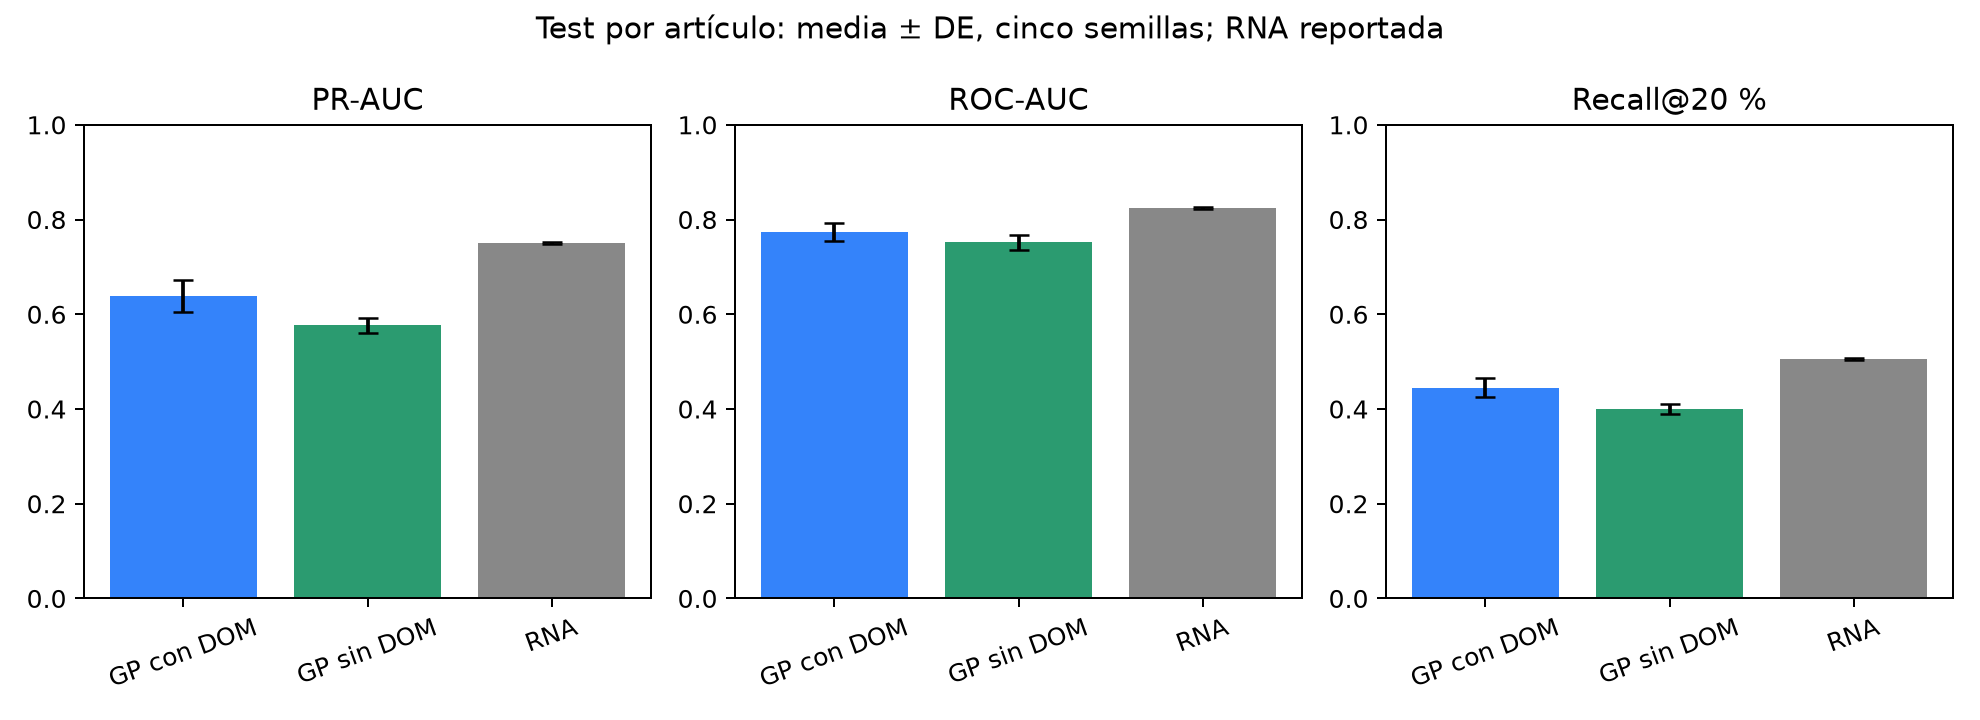
\includegraphics[width=0.72\textwidth]{rna_gp_comparison.png}
\caption{Comparación en el conjunto de prueba, por artículo: media y
desviación estándar sobre cinco semillas del GP con y sin \col{DOM_DOMAIN_ID},
frente a la RNA reportada sobre el mismo mes de prueba.}
\label{fig:comparacion}
\end{figure*}

\section{Impactos éticos y sociales}

\textbf{Correlación, no causalidad.} Las variables de mayor peso en el árbol
de referencia son tasas históricas de pérdida por dominio, instalación y
marca. Un puntaje alto no indica que la instalación o el vendedor sean
responsables; refleja el historial agregado de una categoría. El agente se
plantea como apoyo a la priorización humana y nunca como mecanismo automático
de sanción a instalaciones, vendedores o transportistas.

\textbf{Sesgo heredado y artefactos de extracción.} Si la base histórica
contiene artefactos, el modelo los reproduce con apariencia de evidencia. El
caso de \col{LG_REGION} ya demostró que una taxonomía puede codificar la
etiqueta; la sospecha equivalente sobre \col{DOM_DOMAIN_ID} (seis valores con
100\,\% de pérdida y 200 a 834 filas cada uno en el conjunto completo; tres
categorías grandes y puras con 1\,507 filas, el 1,2\,\% del entrenamiento, en
la auditoría de esta corrida) implica que el agente podría marcar
sistemáticamente productos de ciertas categorías por un defecto de la
extracción y no por un riesgo real. La interpretabilidad del GP ayuda: el peso
del dominio es visible en la fórmula y la ablación lo cuantifica. Esa
transparencia obliga, no exime, a investigar el artefacto antes de operar.

\textbf{Confidencialidad y efecto sobre la revisión.} Los mapas de
codificación contienen categorías, marcas e instalaciones de la empresa, por
lo que los modelos entrenados se conservan solo localmente y se excluyen del
paquete compartible; los archivos agregados no contienen identificadores de
envío. Además, una lista priorizada concentra la atención en una fracción de
los envíos: con Recall@20\,\% de 0,445, más de la mitad de las pérdidas
quedarían fuera de la revisión, y el puntaje debe complementar, no sustituir,
los controles existentes.

\section{Resultados y criterios de comparación}

\textbf{Desempeño predictivo.} La RNA es superior en todas las métricas de
orden: 0,110 más de PR-AUC y 0,051 más de ROC-AUC en media, diferencias que
superan con holgura la dispersión entre semillas de ambos modelos. El GP sin
dominio queda 0,173 por debajo en PR-AUC. El mejor árbol individual (semilla
44, PR-AUC 0,689) tampoco alcanza la peor semilla de la RNA.

\textbf{Calidad de la priorización.} El GP captura menos pérdidas en cada
fracción revisada (Recall@20\,\% de 0,445 frente a 0,506) y con menos
precisión en la cima (Precision@10\,\% de 0,810 frente a 0,942). Sin embargo,
la Precision@1\,\% perfecta de la RNA, que el GP reproduce solo en la semilla
46, es justamente la cifra bajo sospecha por el artefacto de dominio; la
ventaja de la RNA en la cima podría estar inflada por la misma variable que el
GP pondera con el mayor coeficiente.

\textbf{Interpretabilidad.} Es el criterio en el que el GP gana sin discusión.
Los modelos finales tienen entre 7 y 36 nodos (media 20,6~$\pm$~11,6 con
dominio); el de referencia se reduce a una suma ponderada de siete terminales
y el de la ablación a una regla lineal de cinco. Un revisor puede leer por qué
un envío quedó arriba; la RNA, un ensamble de dos redes con
\textit{embeddings}, solo ofrece importancias por permutación a posteriori.
Debe matizarse que los terminales son variables transformadas (tasas
históricas y frecuencias aprendidas en entrenamiento), no las columnas crudas:
la fórmula es legible, pero no es una ecuación directa sobre pesos y montos.

\textbf{Costo computacional.} Sin los intervalos anómalos, una corrida del GP
tarda entre 50 y 85~s en CPU, comparable con la RNA; el GP no requiere GPU ni
la pila de AutoGluon, pero el cribado añadió seis corridas. Ninguna técnica
tiene una ventaja de velocidad demostrada.

\textbf{Estabilidad entre semillas.} La RNA es muy estable (desviación de
PR-AUC de 0,0020); el GP varía 0,0338 con dominio y 0,0160 sin él, y sus
árboles cambian de forma y tamaño entre semillas (de 9 a 36 nodos). La
búsqueda con 180 individuos y 25 generaciones no converge a una misma
solución, lo que es esperable en regresión simbólica y exige reportar varias
semillas.

\textbf{Dependencia de \col{DOM_DOMAIN_ID}.} Ambos modelos dependen del
dominio: es la variable más importante de la RNA (caída de PR-AUC de 0,197 al
permutarla~\cite{informe_rna}) y la de mayor coeficiente en el árbol de
referencia; su ablación en el GP cuesta 0,0626 de PR-AUC. La ablación muestra
dependencia, no causalidad, y no prueba la ausencia de otros artefactos:
categorías correlacionadas pueden conservar una señal similar.

\section{Conclusiones y trabajo futuro}

Un clasificador simbólico evolucionado con programación genética, entrenado
solo con información disponible al crear el envío y bajo el mismo protocolo
temporal que la red neuronal, ordena el riesgo de pérdida de forma útil
(PR-AUC de 0,639~$\pm$~0,034 frente a 0,312 del azar; ROC-AUC de
0,773~$\pm$~0,019) pero no alcanza a la RNA (0,750 y 0,824) en ningún criterio
de desempeño. A cambio ofrece un modelo de decenas de nodos que puede leerse y
auditarse, y que hace explícita la dependencia de la variable de dominio que
en la RNA solo se infiere por permutación. La respuesta a la pregunta del
módulo es parcial: el GP es interpretable, pero no competitivo en precisión
con la configuración y el presupuesto evaluados.

El resultado más valioso vuelve a ser metodológico. Mantener la selección de
configuración, árbol y umbral exclusivamente en validación, sellarla antes de
puntuar la prueba, repetir cinco semillas y validar de forma independiente que
las etiquetas y las columnas de fuga no alteran los puntajes permite afirmar
que la brecha con la RNA es real y no un artefacto de la evaluación. La mejora
frente a la prueba inicial del GP (PR-AUC 0,548, una semilla) cambió a la vez
codificación, presupuesto y filas de aptitud, y no es atribuible a una sola
técnica.

El trabajo futuro inmediato es auditar \col{DOM_DOMAIN_ID} en la fuente, pues
condiciona a ambos modelos; ampliar la búsqueda de hiperparámetros del GP con
más semillas por configuración y presupuestos mayores, cuyo límite no se
alcanzó; probar primitivas condicionales y una aptitud multiobjetivo que
explicite el compromiso entre PR-AUC y tamaño; evaluar la disponibilidad real
de las etiquetas históricas que asume la codificación temporal; y agregar
métricas a nivel de envío y meses de prueba adicionales, lo que requiere una
nueva extracción homogénea. Las técnicas restantes del proyecto, inferencia
difusa y métodos de ensamble, se evaluarán con este mismo protocolo; un
ensamble que combine la RNA con el árbol simbólico es un candidato natural
para unir desempeño e interpretabilidad.

\begin{thebibliography}{00}
\bibitem{meli10k} MercadoLibre, Inc., ``Annual Report on Form 10-K for the
fiscal year ended December 31, 2025,'' U.S. Securities and Exchange
Commission, 25 feb. 2026.
\bibitem{bortolini} M. Bortolini \textit{et al.}, ``A deep learning approach to
predict supply chain delivery delay risk based on macroeconomic indicators: A
case study in the automotive sector,'' \textit{Applied Sciences}, vol. 14,
no. 11, art. 4688, 2024, doi: 10.3390/app14114688.
\bibitem{nezamoddini} N. Nezamoddini, A. Gholami y F. Aqlan, ``A risk-based
optimization framework for integrated supply chains using genetic algorithm
and artificial neural networks,'' \textit{Int. J. Production Economics},
art. 107569, 2020, doi: 10.1016/j.ijpe.2019.107569.
\bibitem{gajovic} V. Gajović, M. Kerkez y J. Kočović, ``Modeling and
simulation of logistic processes: Risk assessment with a fuzzy logic
technique,'' \textit{Simulation}, vol. 94, no. 6, 2018,
doi: 10.1177/0037549717738351.
\bibitem{ifac2022} ``Delay prediction to mitigate e-commerce supplier
disruptions using voting mechanism,'' \textit{IFAC-PapersOnLine}, vol. 55,
no. 10, pp. 731--736, 2022, doi: 10.1016/j.ifacol.2022.09.495.
\bibitem{aqlan} F. Aqlan y S. S. Lam, ``A fuzzy-based integrated framework for
supply chain risk assessment,'' \textit{Int. J. Production Economics},
vol. 161, pp. 54--63, 2015, doi: 10.1016/j.ijpe.2014.11.013.
\bibitem{ye} B. Ye, J. Zuo, X. Zhao y L. Luo, ``Research on the express
delivery delay prediction based on neural network in the background of big
data,'' en \textit{Proc. 6th Int. Conf. Electronic, Mechanical, Information
and Management Society}, 2016, pp. 1449--1454, doi: 10.2991/emim-16.2016.294.
\bibitem{koza} J. R. Koza, \textit{Genetic Programming: On the Programming of
Computers by Means of Natural Selection}. Cambridge, MA, EE.~UU.: MIT Press,
1992.
\bibitem{deap} F.-A. Fortin, F.-M. De Rainville, M.-A. Gardner, M. Parizeau y
C. Gagné, ``DEAP: Evolutionary algorithms made easy,'' \textit{J. Machine
Learning Research}, vol. 13, pp. 2171--2175, 2012.
\bibitem{saito} T. Saito y M. Rehmsmeier, ``The precision-recall plot is more
informative than the ROC plot when evaluating binary classifiers on imbalanced
datasets,'' \textit{PLoS ONE}, vol. 10, no. 3, art. e0118432, 2015.
\bibitem{informe_rna} K. Bueno S. y L. Portela L., ``RiskShip: Priorización
inteligente de envíos con riesgo de falla. Solución con redes neuronales,''
informe de proyecto, Pontificia Universidad Javeriana, Bogotá, 2026.
\bibitem{espejo} P. G. Espejo, S. Ventura y F. Herrera, ``A survey on the
application of genetic programming to classification,'' \textit{IEEE Trans.
Syst., Man, Cybern. C, Appl. Rev.}, vol. 40, no. 2, pp. 121--144, 2010,
doi: 10.1109/TSMCC.2009.2033566.
\bibitem{bhowan2012} U. Bhowan, M. Johnston y M. Zhang, ``Developing new
fitness functions in genetic programming for classification with unbalanced
data,'' \textit{IEEE Trans. Syst., Man, Cybern. B, Cybern.}, vol. 42, no. 2,
pp. 406--421, 2012, doi: 10.1109/TSMCB.2011.2167144.
\bibitem{bhowan2013} U. Bhowan, M. Johnston, M. Zhang y X. Yao, ``Evolving
diverse ensembles using genetic programming for classification with
unbalanced data,'' \textit{IEEE Trans. Evol. Comput.}, vol. 17, no. 3,
pp. 368--386, 2013, doi: 10.1109/TEVC.2012.2199119.
\bibitem{luke} S. Luke y L. Panait, ``A comparison of bloat control methods
for genetic programming,'' \textit{Evolutionary Computation}, vol. 14, no. 3,
pp. 309--344, 2006, doi: 10.1162/evco.2006.14.3.309.
\bibitem{poli} R. Poli, W. B. Langdon y N. F. McPhee, \textit{A Field Guide
to Genetic Programming}. Lulu.com, 2008, ISBN 978-1-4092-0073-4.
\bibitem{rudin} C. Rudin, ``Stop explaining black box machine learning models
for high stakes decisions and use interpretable models instead,''
\textit{Nature Machine Intelligence}, vol. 1, no. 5, pp. 206--215, 2019,
doi: 10.1038/s42256-019-0048-x.
\bibitem{lacava} W. La Cava \textit{et al.}, ``Contemporary symbolic
regression methods and their relative performance,'' en \textit{Proc. NeurIPS
Datasets and Benchmarks Track}, 2021, doi: 10.48550/arXiv.2107.14351.
\bibitem{grinsztajn} L. Grinsztajn, E. Oyallon y G. Varoquaux, ``Why do
tree-based models still outperform deep learning on typical tabular data?,''
en \textit{Advances in Neural Information Processing Systems}, vol. 35, 2022,
doi: 10.48550/arXiv.2207.08815.
\bibitem{shwartz} R. Shwartz-Ziv y A. Armon, ``Tabular data: Deep learning is
not all you need,'' \textit{Information Fusion}, vol. 81, pp. 84--90, 2022,
doi: 10.1016/j.inffus.2021.11.011.
\bibitem{davis} J. Davis y M. Goadrich, ``The relationship between
precision-recall and ROC curves,'' en \textit{Proc. 23rd Int. Conf. Machine
Learning (ICML)}, 2006, pp. 233--240, doi: 10.1145/1143844.1143874.
\bibitem{kaufman} S. Kaufman, S. Rosset, C. Perlich y O. Stitelman, ``Leakage
in data mining: Formulation, detection, and avoidance,'' \textit{ACM Trans.
Knowl. Discov. Data}, vol. 6, no. 4, art. 15, pp. 1--21, 2012,
doi: 10.1145/2382577.2382579.
\bibitem{deleeuw} J. de Leeuw, Z. Bukhsh y Y. Zhang, ``Parcel loss prediction
in last-mile delivery: Deep and non-deep approaches with insights from
explainable AI,'' preimpresión arXiv:2310.16602, 2023,
doi: 10.48550/arXiv.2310.16602.
\bibitem{zhang2026} Y. Zhang, Y. Wang y Y. Wang, ``A deep tabular learning
framework for e-commerce delivery delay prediction and cost-sensitive
operational risk mitigation,'' \textit{Algorithms}, vol. 19, no. 7, art. 597,
2026, doi: 10.3390/a19070597.
\bibitem{lunet} M. Lunet, D. Fernandes, F. Neves-Moreira y P. Amorim,
``Symbolic pricing policies for attended home delivery -- the case of an
online retailer,'' en \textit{Proc. Genetic and Evolutionary Computation
Conf. (GECCO)}, 2025, pp. 1397--1405, doi: 10.1145/3712256.3726361.
\end{thebibliography}

\end{document}
